% !TEX program = xelatex
\documentclass[14pt,a4paper,oneside]{extreport}
% Layout and typography for XeLaTeX
\usepackage{fontspec}
\usepackage{polyglossia}
\setdefaultlanguage{russian}
\setotherlanguage{english}
\IfFontExistsTF{PT Serif}{\setmainfont{PT Serif}}{\setmainfont{TeX Gyre Termes}}
\IfFontExistsTF{PT Sans}{\setsansfont{PT Sans}}{\setsansfont{TeX Gyre Heros}}
\IfFontExistsTF{PT Mono}{\setmonofont{PT Mono}}{\setmonofont{TeX Gyre Cursor}}
\usepackage[a4paper,left=30mm,right=10mm,top=20mm,bottom=20mm]{geometry}
\usepackage{setspace}
\onehalfspacing
\usepackage{indentfirst}
\setlength{\parindent}{1.25cm}
\setlength{\parskip}{0pt}
\usepackage{graphicx}
\graphicspath{{figures/}}
\usepackage{float}
\usepackage{booktabs,longtable,array,tabularx,makecell,calc}
\usepackage{caption}
\captionsetup{font=normalsize,labelfont=bf,justification=centering,singlelinecheck=false}
\usepackage{listings}
\usepackage{xcolor}
\lstdefinestyle{pythoncourse}{
  language=Python,
  basicstyle=\ttfamily\fontsize{8.5}{10}\selectfont,
  keywordstyle=\bfseries,
  commentstyle=\itshape,
  stringstyle=\ttfamily,
  numbers=left,
  numberstyle=\tiny,
  stepnumber=1,
  numbersep=7pt,
  frame=single,
  breaklines=true,
  breakatwhitespace=false,
  showstringspaces=false,
  tabsize=4,
  columns=fullflexible,
  keepspaces=true,
  xleftmargin=1em,
  framexleftmargin=0.5em,
  aboveskip=0.5\baselineskip,
  belowskip=0.5\baselineskip
}
\lstset{style=pythoncourse}
\newenvironment{listingblock}{\par\smallskip\begin{minipage}{\linewidth}}{\end{minipage}\par\smallskip}
\usepackage{titlesec}
\renewcommand{\chaptername}{Глава}
\titleformat{\chapter}[block]{\centering\bfseries\fontsize{16}{19}\selectfont}{\chaptername\ \thechapter.}{0.5em}{}
\titlespacing*{\chapter}{0pt}{-8pt}{24pt}
\titleformat{\section}[block]{\centering\bfseries\fontsize{14}{17}\selectfont}{\thesection.}{0.5em}{}
\titlespacing*{\section}{0pt}{18pt}{12pt}
\titleformat{\subsection}[block]{\bfseries\fontsize{14}{17}\selectfont}{\thesubsection.}{0.5em}{}
\titlespacing*{\subsection}{0pt}{14pt}{8pt}
\usepackage{tocloft}
\renewcommand{\contentsname}{Оглавление}
\renewcommand{\cftchapfont}{\bfseries}
\renewcommand{\cftchappagefont}{\bfseries}
\renewcommand{\cftsecfont}{\bfseries}
\renewcommand{\cftsecpagefont}{\bfseries}
\setlength{\cftbeforechapskip}{5pt}
\setcounter{secnumdepth}{2}
\setcounter{tocdepth}{2}
\usepackage{fancyhdr}
\fancyhf{}
\fancyfoot[C]{\thepage}
\renewcommand{\headrulewidth}{0pt}
\renewcommand{\footrulewidth}{0pt}
\pagestyle{fancy}
\fancypagestyle{plain}{\fancyhf{}\fancyfoot[C]{\thepage}\renewcommand{\headrulewidth}{0pt}}
\usepackage{xurl}
\usepackage{hyperref}
\hypersetup{hidelinks,pdftitle={Курсовой проект: генерация названий растений и продуктов},pdfauthor={Жаринов К. С.}}
\usepackage{microtype}
\emergencystretch=2em


% Данные титульного листа. При необходимости измените их здесь.
\newcommand{\StudentName}{Жаринов К. С.}
\newcommand{\StudentGroup}{Д-Э 21-24}
\newcommand{\StudentCourse}{3 курса}
\newcommand{\CourseTitle}{Разработка методов машинного обучения для генерации названий растений и аграрных объектов виртуальных миров}
\newcommand{\InstituteName}{Институт экономики и управления}
\newcommand{\DepartmentName}{Кафедра статистики и кибернетики}
\newcommand{\DirectionName}{09.03.02 Информационные системы и технологии}
\newcommand{\ProfileName}{Большие данные и машинное обучение}

\begin{document}
\begin{titlepage}
\thispagestyle{empty}
\begin{center}
\begin{minipage}[c]{0.15\textwidth}
\centering
\IfFileExists{figures/university_logo.png}{
\includegraphics[width=1.75cm]{university_logo.png}}{}
\end{minipage}\hfill
\begin{minipage}[c]{0.83\textwidth}
\centering
\fontsize{7.5}{8.8}\selectfont
МИНИСТЕРСТВО СЕЛЬСКОГО ХОЗЯЙСТВА РОССИЙСКОЙ ФЕДЕРАЦИИ\\
ФЕДЕРАЛЬНОЕ ГОСУДАРСТВЕННОЕ БЮДЖЕТНОЕ ОБРАЗОВАТЕЛЬНОЕ УЧРЕЖДЕНИЕ ВЫСШЕГО ОБРАЗОВАНИЯ\\
«РОССИЙСКИЙ ГОСУДАРСТВЕННЫЙ АГРАРНЫЙ УНИВЕРСИТЕТ -- МСХА имени К. А. ТИМИРЯЗЕВА»\\
(ФГБОУ ВО РГАУ -- МСХА имени К. А. Тимирязева)
\end{minipage}
\end{center}
\vspace{0.12cm}
\hrule height 0.5pt
\vspace{0.42cm}
\begin{center}
{\fontsize{12}{14}\selectfont \InstituteName\\[0.08cm]
\DepartmentName\par}
\vspace{0.35cm}
{\fontsize{12}{14}\selectfont Направление: \DirectionName\\
Направленность:\\
\ProfileName\par}
\vspace{0.55cm}
{\bfseries\fontsize{17}{20}\selectfont КУРСОВОЙ ПРОЕКТ\par}
\end{center}
\vspace{0.18cm}
{\fontsize{12}{14}\selectfont на тему: «\CourseTitle»\par}
\vspace{0.35cm}
\begin{flushright}
\begin{minipage}[t]{0.53\textwidth}
\fontsize{10.5}{12.2}\selectfont
Выполнил:\\
Студент \StudentCourse{} группы \StudentGroup\\
\StudentName\par
\vspace{0.22cm}
Дата регистрации КП\\
на кафедре: \rule{5.2cm}{0.4pt}\par
\vspace{0.22cm}
Допущен к защите\\
Руководитель:\par
\vspace{0.25cm}
\rule{5.2cm}{0.4pt}\\[-1pt]
{\fontsize{8.5}{9.5}\selectfont учёная степень, учёное звание, ФИО\par}
\vspace{0.25cm}
Члены комиссии:\par
\vspace{0.12cm}
\rule{3.65cm}{0.4pt}\hspace{0.18cm}\rule{1.05cm}{0.4pt}\\[-1pt]
{\fontsize{8}{9}\selectfont учёная степень, учёное звание, ФИО\hspace{0.25cm}подпись\par}
\vspace{0.12cm}
\rule{3.65cm}{0.4pt}\hspace{0.18cm}\rule{1.05cm}{0.4pt}\\[-1pt]
{\fontsize{8}{9}\selectfont учёная степень, учёное звание, ФИО\hspace{0.25cm}подпись\par}
\vspace{0.12cm}
\rule{3.65cm}{0.4pt}\hspace{0.18cm}\rule{1.05cm}{0.4pt}\\[-1pt]
{\fontsize{8}{9}\selectfont учёная степень, учёное звание, ФИО\hspace{0.25cm}подпись\par}
\vspace{0.25cm}
{\fontsize{10.5}{12}\selectfont Оценка \rule{4.2cm}{0.4pt}\par}
\vspace{0.18cm}
{\fontsize{10.5}{12}\selectfont Дата защиты \rule{3.6cm}{0.4pt}\par}
\end{minipage}
\end{flushright}
\vfill
\begin{center}{\fontsize{11}{13}\selectfont Москва 2026}\end{center}
\end{titlepage}

\pagenumbering{arabic}
\setcounter{page}{2}
\tableofcontents
\clearpage
\chapter*{Введение}\label{ux432ux432ux435ux434ux435ux43dux438ux435}
\addcontentsline{toc}{chapter}{Введение}

В индустрии видеоигр и сельскохозяйственных симуляторов постоянно возникает потребность в большом количестве названий: сортов растений, пород животных, продуктов и географических объектов. Ручное создание такого объёма наименований требует времени и нередко приводит к повторам. Автоматическая генерация позволяет получать новые варианты с заданными свойствами и единым стилем.

Актуальность темы связана с распространением генеративных моделей в обработке естественного языка и потребностью в инструментах нейминга для аграрной и игровой сфер. Для применения LSTM и трансформеров к названиям растений и продуктов необходимо адаптировать архитектуру, подготовить предметный датасет и определить критерии оценки. Это требует понимания принципов работы моделей и их ограничений.

Целью курсового проекта является разработка и исследование методов машинного обучения для генерации названий растений и аграрных объектов виртуальных миров, а также создание программного приложения, реализующего генеративный пайплайн и обеспечивающего удобный пользовательский интерфейс.

Для достижения поставленной цели необходимо решить следующие задачи:

Провести теоретический анализ генеративных моделей машинного обучения, применяемых для генерации текстовых последовательностей, включая рекуррентные нейронные сети (LSTM) и трансформеры.

Изучить методы оценки качества сгенерированных названий: перплексию, стилевое соответствие, новизну и разнообразие.

Обосновать выбор инструментов и разработать архитектуру программного приложения для генерации названий растений и продуктов.

Сформировать и подготовить датасет названий растений и продуктов, включающий разметку по категориям и длине названия.

Реализовать на языке Python генеративную LSTM-модель, классификатор стилей и модули скоринга, а также создать пользовательский интерфейс на базе Gradio.

Провести экспериментальное исследование качества обученных моделей, сравнить результаты с базовыми методами (марковские цепи, n-граммы) и проанализировать полученные данные.

Сформулировать выводы о целесообразности применения выбранных методов для задачи генерации названий в аграрной предметной области.

Объект исследования -- методы машинного обучения для генерации текстовых последовательностей; предмет -- архитектура, обучение и оценка генеративных моделей. Методы: анализ литературы, сравнение архитектур, проектирование и экспериментальное тестирование.

\chapter{Теоретическая часть}\label{ux442ux435ux43eux440ux435ux442ux438ux447ux435ux441ux43aux430ux44f-ux447ux430ux441ux442ux44c}

\section{Понятие генеративных моделей в машинном обучении}\label{ux43fux43eux43dux44fux442ux438ux435-ux433ux435ux43dux435ux440ux430ux442ux438ux432ux43dux44bux445-ux43cux43eux434ux435ux43bux435ux439-ux432-ux43cux430ux448ux438ux43dux43dux43eux43c-ux43eux431ux443ux447ux435ux43dux438ux438}

Машинное обучение представляет собой раздел искусственного интеллекта, посвящённый разработке алгоритмов, способных извлекать закономерности из данных и применять их к новым, ранее не встречавшимся примерам {[}19, 20{]}. В зависимости от характера решаемой задачи методы машинного обучения принято делить на несколько крупных классов: обучение с учителем, обучение без учителя, обучение с подкреплением и генеративное обучение. Каждый из этих классов имеет собственные принципы построения моделей и собственные критерии качества.

При обучении с учителем модель получает примеры с правильными ответами. Обучение без учителя предполагает самостоятельный поиск структур и кластеров в данных, а обучение с подкреплением строится на взаимодействии со средой и получении награды или штрафа.

Генеративное обучение занимает в этой классификации особое место. Его задача -- не предсказать ответ по входным данным, а научиться порождать новые данные, похожие на те, что были в обучающей выборке {[}1, 13{]}. Иными словами, модель должна усвоить вероятностное распределение данных и затем уметь извлекать из него новые примеры. Если модель обучена на фотографиях кошек, она должна уметь генерировать новые фотографии кошек, которых никогда не было, но которые выглядят правдоподобно.

Классический пример генеративной модели -- GAN, предложенная И. Гудфеллоу и соавторами в 2014 году {[}13{]}. Она объединяет генератор, создающий образцы, и дискриминатор, отличающий их от реальных. Соревнование сетей постепенно повышает качество генерации. GAN широко применяются для изображений, видео и звука, но менее удобны для текста из-за его дискретной природы.

Языковые модели оценивают вероятность последовательностей символов или слов и порождают новые последовательности {[}5, 17{]}. Развитие этого направления прошло путь от частотных n-граммных моделей к рекуррентным сетям и трансформерам {[}5, 11{]}. Большие языковые модели, например GPT, создают связный текст, но требуют значительных вычислительных ресурсов и больших обучающих корпусов {[}18{]}.

В данной работе рассматриваются посимвольные языковые модели для генерации коротких последовательностей -- названий. Они не требуют токенизации, могут обучаться на сравнительно небольших датасетах и запускаться на обычном компьютере. Это делает их подходящими для узкой предметной области растений и продуктов.

Обучение и инференс -- разные этапы работы генеративной модели. При обучении параметры корректируются на примерах из датасета; при инференсе уже обученная модель создаёт новые последовательности. В работе обучение выполняется локально, а генерация доступна через приложение.

\section{Задача генерации текстовых последовательностей}\label{ux437ux430ux434ux430ux447ux430-ux433ux435ux43dux435ux440ux430ux446ux438ux438-ux442ux435ux43aux441ux442ux43eux432ux44bux445-ux43fux43eux441ux43bux435ux434ux43eux432ux430ux442ux435ux43bux44cux43dux43eux441ux442ux435ux439}

Генерация текста заключается в построении модели, которая по обучающим примерам создаёт новые статистически похожие последовательности {[}4, 5{]}. Для названий растений и продуктов важно, чтобы результат был правдоподобным, соответствовал выбранной категории и не повторял примеры корпуса.

Один из первых подходов -- n-граммные модели, оценивающие частоты соседних символов или слов {[}5, 10{]}. Модель порядка n учитывает предыдущие n−1 элементов и на их основе выбирает следующий. Например, биграммная модель использует пары соседних символов, поэтому её работу легко понять и проверить.

Недостаток n-грамм -- слабая работа с редкими сочетаниями: если нужный переход не встречался, оценить его вероятность трудно. Сглаживание Кнесера -- Нея перераспределяет вероятности и даёт небольшую вероятность редким сочетаниям {[}10{]}.

При увеличении n число возможных контекстов быстро растёт, а данных для их оценки не хватает. Поэтому на практике используют небольшие порядки, что ограничивает учёт дальнего контекста.

Нейросетевые языковые модели заменили таблицы частот обучаемыми векторными представлениями и сетями, которые выявляют закономерности сочетания символов и слов {[}5, 15, 16{]}. Модель Бенджио и соавторов 2003 года стала одним из ранних примеров такого подхода {[}5{]}.

Посимвольные модели рассматривают название как последовательность отдельных знаков. Такой подход не требует словаря готовых слов и позволяет получать неологизмы {[}7, 16{]}. Его недостаток -- большее число шагов по сравнению со словесной моделью, что увеличивает вычислительную нагрузку.

Генерация носит вероятностный характер: на каждом шаге следующий символ выбирается из распределения вероятностей. Благодаря этому одна модель создаёт разные варианты. Степень случайности регулируется параметрами сэмплирования.

Качество генерации оценивают количественно -- по перплексии, новизне и разнообразию -- и качественно, с помощью экспертной оценки. Поскольку единственного правильного ответа нет, метрики рассматриваются совместно; подробнее они описаны в разделе 1.5.

\section{Рекуррентные нейронные сети и архитектура LSTM}\label{ux440ux435ux43aux443ux440ux440ux435ux43dux442ux43dux44bux435-ux43dux435ux439ux440ux43eux43dux43dux44bux435-ux441ux435ux442ux438-ux438-ux430ux440ux445ux438ux442ux435ux43aux442ux443ux440ux430-lstm}

Рекуррентные нейронные сети (RNN) предназначены для обработки последовательностей {[}1, 6{]}. Их скрытое состояние передаётся между шагами, поэтому при обработке текущего символа сеть учитывает предшествующий контекст. В отличие от полносвязных сетей, элементы последовательности не рассматриваются независимо.

На каждом шаге RNN получает текущий символ и предыдущее скрытое состояние, а возвращает новое состояние и прогноз следующего символа. В скрытом состоянии сохраняется информация о ранее обработанной части последовательности.

Простые RNN подвержены затуханию и взрыву градиента {[}6{]}. При обратном распространении ошибки через много временных шагов градиенты могут становиться слишком малыми или слишком большими. В результате сеть забывает дальний контекст либо обучается нестабильно.

Решением проблемы стала архитектура LSTM (Long Short-Term Memory, «долгая краткосрочная память»), предложенная в 1997 году З. Хохрайтером и Ю. Шмидхубером {[}6{]}. LSTM сохраняет общую идею рекуррентной обработки, но вводит более сложную внутреннюю структуру ячейки, способную эффективно сохранять и передавать информацию на длинные дистанции.

Ключевым элементом LSTM является наличие двух состояний: скрытого состояния (как в обычной RNN) и так называемого состояния ячейки (cell state). Состояние ячейки представляет собой долговременную память, которая может беспрепятственно переноситься через многие шаги с минимальными изменениями. Управление этой памятью осуществляется с помощью трёх специальных механизмов, называемых «вентилями» (gates): вентиля забывания, входного вентиля и выходного вентиля.

Вентиль забывания определяет, какую информацию из предыдущего состояния сохранить. Входной вентиль регулирует запись новых сведений, а выходной -- передачу части состояния ячейки в скрытое состояние для прогноза следующего символа.

Благодаря такой структуре LSTM может сохранять важные сведения на протяжении многих шагов и отбрасывать несущественные. Архитектура применялась для языкового моделирования {[}15{]}, генерации текста {[}7, 16{]}, машинного перевода и распознавания речи.

В контексте генерации названий LSTM работает следующим образом. На вход модели подаётся начало названия (или специальный маркер начала). На каждом шаге модель предсказывает распределение вероятностей по всем возможным символам и выбирает один из них. Выбранный символ добавляется к последовательности и подаётся на вход на следующем шаге. Процесс повторяется до тех пор, пока не будет сгенерирован специальный маркер конца или не будет достигнута максимальная длина.

Для условной генерации в модель дополнительно передаются категория названия и требуемое количество слов. Их векторные представления объединяются с символьными эмбеддингами и подаются на вход LSTM. Благодаря этому модель учитывает запрос пользователя, например генерирует названия именно для ягод или зерновых.

Кроме того, при обучении LSTM применяются стандартные методы регуляризации -- в частности, dropout {[}14{]}, который случайным образом «выключает» часть нейронов во время обучения, что помогает предотвратить переобучение. Используется также оптимизатор Adam {[}12{]} -- адаптивный метод градиентного спуска, хорошо зарекомендовавший себя в задачах обучения нейронных сетей.

Хотя трансформеры получили широкое распространение {[}11{]}, LSTM остаётся практичным выбором для небольших задач. Такие модели компактны, обучаются на CPU и требуют сравнительно небольшого датасета, что соответствует условиям настоящей работы.

Таким образом, LSTM сочетает последовательную обработку с механизмом долговременной памяти и подходит для генерации коротких названий. Далее рассматривается альтернативная архитектура -- трансформер.

\section{Трансформеры и механизм внимания}\label{ux442ux440ux430ux43dux441ux444ux43eux440ux43cux435ux440ux44b-ux438-ux43cux435ux445ux430ux43dux438ux437ux43c-ux432ux43dux438ux43cux430ux43dux438ux44f}

Архитектура LSTM, рассмотренная в предыдущем разделе, долгое время оставалась основной для задач обработки последовательностей. Однако у неё есть принципиальное ограничение: обработка последовательности происходит строго последовательно, шаг за шагом. Это затрудняет распараллеливание вычислений и ограничивает длину контекста, который модель может эффективно учитывать. Решением этой проблемы стала архитектура трансформера, предложенная в 2017 году группой исследователей из Google под руководством А. Васвани {[}11{]}.

Ключевой идеей трансформера является механизм внимания (attention mechanism) -- специальный способ обработки последовательности, при котором каждый элемент может напрямую «взаимодействовать» с любым другим элементом, независимо от их взаимного расположения. В отличие от рекуррентных сетей, где информация передаётся последовательно через скрытые состояния, в трансформере каждый элемент «видит» всю последовательность целиком и сам решает, на какие элементы обратить внимание.

Механизм внимания удобно представить следующим образом. Для каждого элемента последовательности вычисляются три векторных представления: запрос (query), ключ (key) и значение (value). Запрос описывает, что именно ищет текущий элемент; ключ -- что может предложить каждый элемент; значение -- какую информацию несёт каждый элемент. Затем для текущего элемента вычисляется степень его соответствия каждому элементу последовательности -- насколько его запрос «подходит» к ключам других элементов. По этим степеням формируются веса, с которыми значения других элементов суммируются и добавляются к представлению текущего элемента. В результате каждый элемент получает «сжатую» информацию обо всей последовательности, взвешенную по релевантности.

Такая схема получила название self-attention (самовнимание), поскольку запросы, ключи и значения вычисляются из одной и той же последовательности. Она позволяет модели гибко учитывать контекст: например, при обработке названия «Пшеница Озимая» модель может «обратить внимание» на связь между первым и вторым словом, чтобы правильно определить род прилагательного.

Одним из важных усовершенствований механизма внимания является многоголовое внимание (multi-head attention). Идея в том, что вместо одной «головы» внимания используется несколько параллельных «голов», каждая из которых фокусируется на своём аспекте последовательности. Например, одна голова может отслеживать синтаксические связи, другая -- фонетические паттерны, третья -- семантические. Результаты всех голов затем объединяются. Это делает модель более выразительной и устойчивой.

Полноценная архитектура трансформера состоит из энкодера и декодера, каждый из которых содержит несколько слоёв. Слой энкодера включает механизм многоголового self-attention и полносвязную нейронную сеть с нелинейной активацией; слой декодера дополнительно содержит механизм attention между энкодером и декодером. В задачах генерации текста (в том числе генерации названий) чаще используется декодер-only вариант, в котором модель просто предсказывает следующий символ по предыдущим, но делает это с помощью механизма внимания вместо рекуррентности.

По сравнению с LSTM, трансформер обладает несколькими существенными преимуществами. Во-первых, он легко распараллеливается: все позиции обрабатываются одновременно, что позволяет эффективно использовать графические ускорители и обучать очень большие модели. Во-вторых, он лучше справляется с длинными зависимостями: информация между удалёнными элементами передаётся напрямую, без искажений через промежуточные состояния. В-третьих, его архитектура более гибкая: добавляя слои и головы внимания, можно легко масштабировать модель.

Вместе с тем трансформер имеет и недостатки, особенно важные для прикладных задач малого масштаба. Главный из них высокие требования к объёму данных. Из-за большого числа параметров трансформеру нужно гораздо больше примеров для обучения, чем LSTM. На небольших датасетах (несколько сотен или тысяч примеров) трансформер склонен к переобучению и уступает более простым архитектурам. Второй недостаток -- вычислительная стоимость: обучение и инференс трансформера заметно дороже, чем у LSTM, даже при сопоставимом числе параметров.

\textbf{Таблица 1.1 -- Сравнение архитектур LSTM и Трансформер}

\begin{longtable}[]{@{}
  >{\raggedright\arraybackslash}p{(\columnwidth - 4\tabcolsep) * \real{0.3243}}
  >{\raggedright\arraybackslash}p{(\columnwidth - 4\tabcolsep) * \real{0.3243}}
  >{\raggedright\arraybackslash}p{(\columnwidth - 4\tabcolsep) * \real{0.3243}}@{}}
\toprule\noalign{}
\begin{minipage}[b]{\linewidth}\raggedright
\textbf{Критерий}
\end{minipage} & \begin{minipage}[b]{\linewidth}\raggedright
\textbf{LSTM}
\end{minipage} & \begin{minipage}[b]{\linewidth}\raggedright
\textbf{Трансформер}
\end{minipage} \\
\midrule\noalign{}
\endhead
\bottomrule\noalign{}
\endlastfoot
Принцип обработки последовательности & Последовательный (шаг за шагом) & Параллельный (все позиции одновременно) \\
Учёт долгосрочных зависимостей & Через скрытое состояние и вентили & Через механизм внимания напрямую \\
Требования к объёму данных & Умеренные (сотни--тысячи примеров) & Высокие (десятки тысяч примеров) \\
Вычислительная стоимость обучения & Низкая (работает на CPU) & Высокая (желателен GPU) \\
Склонность к переобучению на малых данных & Низкая & Высокая \\
Скорость инференса & Высокая & Средняя \\
Пригодность для малых датасетов & Высокая & Низкая \\
\end{longtable}

Именно поэтому в настоящей курсовой работе основным выбором стала LSTM, а трансформер использовался в качестве альтернативной архитектуры для сравнения. На датасете из нескольких тысяч названий LSTM показала более стабильные результаты и лучше обобщила на новые примеры, тогда как трансформер продемонстрировал склонность к переобучению. Этот вывод согласуется с общей практикой применения нейросетевых моделей: выбор архитектуры определяется не только её теоретической мощностью, но и объёмом доступных данных.

Следует также отметить, что для реальных приложений генерации названий малого масштаба не требуется мощная языковая модель уровня GPT. Как показала практика, компактная LSTM, обученная на нескольких тысячах примеров, способна генерировать качественные и осмысленные названия при минимальных вычислительных затратах. Трансформеры же показывают свои преимущества в задачах с большими объёмами данных и длинными контекстами -- в тех сценариях, где их вычислительная стоимость оправдана.

Таким образом, механизм внимания и архитектура трансформера представляют собой важный этап в развитии методов обработки последовательностей. Они расширяют возможности моделирования долгосрочных зависимостей и обеспечивают высокую производительность на больших данных. Однако для задач малого масштаба, к которым относится генерация названий растений и продуктов, LSTM остаётся более практичным выбором. В следующем разделе будут рассмотрены методы оценки качества сгенерированных названий -- независимо от того, какой архитектурой они получены.

\section{Методы оценки качества сгенерированных названий}\label{ux43cux435ux442ux43eux434ux44b-ux43eux446ux435ux43dux43aux438-ux43aux430ux447ux435ux441ux442ux432ux430-ux441ux433ux435ux43dux435ux440ux438ux440ux43eux432ux430ux43dux43dux44bux445-ux43dux430ux437ux432ux430ux43dux438ux439}

Оценка генеративных моделей сложнее оценки классификаторов: у сгенерированного названия нет единственного правильного ответа. Поэтому для сравнения моделей используются несколько взаимодополняющих метрик: перплексия, стилевое соответствие, новизна, разнообразие и человеческая оценка.

Перплексия (perplexity) показывает, насколько уверенно языковая модель предсказывает последовательность {[}4, 15{]}. Чем ниже значение, тем лучше модель описывает данные. При равномерном случайном выборе символов перплексия близка к размеру словаря, а при идеальном предсказании равна единице.

Перплексия является относительной метрикой: корректно сравнивать её можно только для моделей с одинаковым словарём и датасетом. Она характеризует предсказание последовательностей, но не оценивает эстетическое качество названий.

Стилевое соответствие (style adherence) показывает, насколько результат отвечает заданной категории. Для этого используется классификатор, обученный распознавать категории названий. Оценкой служит вероятность класса, соответствующего запросу пользователя.

Такой способ не требует ручной разметки каждого нового результата: классификатор применяет закономерности, усвоенные на исходном датасете.

Новизна (novelty) показывает, насколько сгенерированное название отличается от обучающих примеров. Для её оценки можно сравнивать символьные n-граммы нового названия с n-граммами корпуса. Чем меньше сходство с существующими названиями, тем выше новизна. При этом полное отсутствие общих фрагментов не всегда означает осмысленность результата, поэтому метрику нельзя использовать отдельно.

Разнообразие (diversity) характеризует различия между названиями, созданными в одной серии. Если модель постоянно повторяет одинаковые или почти одинаковые варианты, разнообразие низкое. Для оценки применяются доля уникальных результатов и расстояния между строками.

Человеческая оценка (human evaluation) остаётся важным способом проверки, хотя требует времени. Несколько респондентов могут оценить естественность, соответствие категории и удобство использования названий.

В настоящей работе такая оценка проводилась в ограниченном объёме: респонденты сравнивали варианты и отмечали наиболее удачные. Результаты использовались как дополнительная качественная проверка.

Для сопоставления также использовались базовые модели -- марковская цепь и n-граммный генератор. Сравнение с ними показывает, даёт ли нейросетевая архитектура практическое преимущество.

Таким образом, качество оценивалось по совокупности языковых, стилевых и сравнительных показателей, а также с помощью человеческой оценки.

\textbf{Таблица 1.2 -- Метрики оценки качества генеративных моделей}

\begin{longtable}[]{@{}
  >{\raggedright\arraybackslash}p{(\columnwidth - 6\tabcolsep) * \real{0.2000}}
  >{\raggedright\arraybackslash}p{(\columnwidth - 6\tabcolsep) * \real{0.2533}}
  >{\raggedright\arraybackslash}p{(\columnwidth - 6\tabcolsep) * \real{0.2400}}
  >{\raggedright\arraybackslash}p{(\columnwidth - 6\tabcolsep) * \real{0.2800}}@{}}
\toprule\noalign{}
\begin{minipage}[b]{\linewidth}\raggedright
\textbf{Метрика}
\end{minipage} & \begin{minipage}[b]{\linewidth}\raggedright
\textbf{Что измеряет}
\end{minipage} & \begin{minipage}[b]{\linewidth}\raggedright
\textbf{Диапазон значений}
\end{minipage} & \begin{minipage}[b]{\linewidth}\raggedright
\textbf{Интерпретация}
\end{minipage} \\
\midrule\noalign{}
\endhead
\bottomrule\noalign{}
\endlastfoot
Перплексия & Уверенность модели в предсказаниях & От 1 до размера словаря & Чем ниже, тем лучше \\
Стилевое соответствие & Доля названий, соответствующих категории & От 0 до 1 & Чем выше, тем лучше \\
Новизна & Доля названий, отсутствующих в датасете & От 0 до 1 & Чем выше, тем лучше \\
Разнообразие & Энтропия распределения символов & От 0 до log₂(размер словаря) & Чем выше, тем лучше \\
Человеческая оценка & Субъективное восприятие респондентов & От 1 до 5 & Чем выше, тем лучше \\
\end{longtable}

\section{Обзор существующих генераторов названий}\label{ux43eux431ux437ux43eux440-ux441ux443ux449ux435ux441ux442ux432ux443ux44eux449ux438ux445-ux433ux435ux43dux435ux440ux430ux442ux43eux440ux43eux432-ux43dux430ux437ux432ux430ux43dux438ux439}

Задача генерации названий имеет давнюю историю и большое число практических реализаций. Можно выделить несколько классов существующих инструментов: от простых генераторов на основе шаблонов до современных нейросетевых сервисов.

Шаблонные генераторы используют заранее подготовленные списки слогов или частей слов. Они просты и быстры, но дают ограниченное разнообразие и слабо учитывают особенности конкретной предметной области.

Марковские генераторы строят последовательности на основе вероятностей перехода между символами. Они способны создавать новые комбинации, однако качество зависит от объёма корпуса и порядка модели; дальние зависимости обычно не учитываются.

N-граммные генераторы со сглаживанием расширяют этот подход за счёт учёта более длинных фрагментов и ненулевых вероятностей редких сочетаний. Тем не менее их возможности ограничены размером обучающего корпуса.

Нейросетевые генераторы используют LSTM или GRU и обучаются предсказывать следующий символ или слово. Они лучше обобщают последовательности и могут учитывать более длинный контекст, но требуют подготовки данных и настройки параметров.

Большие языковые модели (LLM), включая GPT, Claude и LLaMA, способны генерировать связный текст по запросу. Однако для узкой задачи нейминга их использование может быть избыточным: требуется доступ к крупной модели, а результат не всегда соответствует заданным ограничениям без дополнительной фильтрации.

Для игр существуют генераторы фэнтезийных имён и топонимов. Обычно они ориентированы на общий художественный стиль, а не на предметные категории сельского хозяйства и продуктов питания.

Специализированных генераторов названий растений и продуктов немного. Разрабатываемая система ориентирована именно на эту область и позволяет управлять категорией и длиной результата.

\chapter{Практическая часть}\label{ux43fux440ux430ux43aux442ux438ux447ux435ux441ux43aux430ux44f-ux447ux430ux441ux442ux44c}

\section{Цели, задачи и методология практического исследования}\label{ux446ux435ux43bux438-ux437ux430ux434ux430ux447ux438-ux438-ux43cux435ux442ux43eux434ux43eux43bux43eux433ux438ux44f-ux43fux440ux430ux43aux442ux438ux447ux435ux441ux43aux43eux433ux43e-ux438ux441ux441ux43bux435ux434ux43eux432ux430ux43dux438ux44f}

Основной целью практической части данной работы является разработка и исследование программного средства для автоматической генерации названий растений и продуктов питания на основе методов машинного обучения, а также эмпирическая проверка качества полученных моделей. Теоретические положения, изложенные в первой главе, задают общие принципы построения генеративных моделей, однако их применение к конкретной предметной области требует решения целого комплекса инженерных и методологических задач. Абстрактные рассуждения о преимуществах LSTM и трансформеров необходимо перевести в плоскость практической реализации: выбрать архитектуру, подготовить данные, настроить гиперпараметры и объективно измерить результат.

Для достижения поставленной цели были сформулированы и последовательно решены следующие задачи:

Формирование предметной области и списка категорий. Прежде чем приступать к сбору данных, необходимо было определить, какие именно названия будет генерировать система. В качестве предметной области выбраны растения (сельскохозяйственные культуры) и продукты питания. Внутри каждого направления выделены пять категорий, отражающих ключевые подобласти: для растений -- зерновые, овощные, плодовые, травы и ягоды; для продуктов -- молочные, мясные, хлебобулочные, напитки и зерновые продукты. Такое деление позволяет пользователю выбирать не просто «растение» или «продукт», а конкретный тип названия, что делает генерацию более осмысленной.

Сбор и подготовка датасета. На основе открытых источников, справочников и собственных дополнений был сформирован исходный корпус названий. Каждое название отнесено к одной из пяти категорий и размечено по количеству слов (одно, два или три). Проведена очистка данных: удалены дубликаты, исправлены опечатки, приведены к единому регистру. Подготовленный датасет послужил основой для обучения всех последующих моделей.

Аугментация данных. Поскольку исходный корпус оказался сравнительно небольшим (несколько сотен названий на категорию), была применена процедура аугментации -- искусственного расширения датасета за счёт комбинаторики. Для каждого названия, состоящего из одного слова (например, «Пшеница»), были сгенерированы дополнительные варианты путём добавления прилагательных («Пшеница Золотая», «Пшеница Северная» и так далее). Это позволило существенно увеличить объём обучающих данных и улучшить качество генерации.

Реализация генеративной LSTM-модели. На языке Python с использованием библиотеки PyTorch была реализована посимвольная LSTM-модель, генерирующая названия по заданной категории и длине. Модель обучена на подготовленном датасете, для неё подобраны гиперпараметры (размер скрытого состояния, количество слоёв, скорость обучения), проведён контроль переобучения с помощью валидационной выборки и ранней остановки.

Реализация моделей скоринга. Для оценки качества сгенерированных названий реализованы три дополнительные модели: классификатор стилей на основе свёрточной нейронной сети (char-CNN), оценщик правдоподобности на основе биграммной языковой модели и оценщик новизны на основе n-граммного сравнения. Эти модели используются для ранжирования сгенерированных названий, чтобы пользователь видел в первую очередь наиболее качественные варианты.

Разработка пользовательского интерфейса. Создано настольное приложение на базе библиотеки Gradio, предоставляющее удобный интерфейс для генерации названий. Приложение содержит две вкладки -- «Растения» и «Продукты», -- в каждой из которых пользователь может выбрать категорию, длину названия, количество результатов и при желании задать seed для воспроизводимости. Реализованы функции копирования, добавления в избранное и экспорта в текстовый файл.

Проведение экспериментального исследования. Обученные модели протестированы на отложенной выборке, измерены метрики качества: перплексия, точность классификатора стилей, доля новых названий, разнообразие. Проведено сравнение с базовыми моделями (марковская цепь, n-граммы с методом Кнесера -- Нея), а также субъективная оценка сгенерированных названий несколькими независимыми респондентами.

Методология исследования базируется на принципах эмпирического анализа алгоритмов машинного обучения. В качестве основного инструмента выбраны язык программирования Python и библиотека PyTorch. Этот выбор обусловлен рядом причин. Во-первых, PyTorch обладает интуитивно понятным API и позволяет сосредоточиться на логике модели, а не на низкоуровневых деталях. Во-вторых, он хорошо документирован и широко используется как в образовательных, так и в производственных проектах. В-третьих, он обеспечивает достаточную производительность на центральном процессоре, что критически важно для локального приложения, не требующего графического ускорителя.

Работа выполнялась поэтапно. На первом этапе были собраны и подготовлены исходные данные, сформирован корпус названий. На втором этапе проведена аугментация данных и разделение на обучающую, валидационную и тестовую выборки. На третьем этапе реализованы и обучены модели (LSTM-генератор, классификатор стилей, оценщики правдоподобности и новизны). На четвёртом этапе разработан пользовательский интерфейс и реализован пайплайн генерации, объединяющий все модели в единую систему. Наконец, на пятом, аналитическом, этапе проведены замеры качества, сравнение с бейзлайнами и интерпретация результатов.

Важно подчеркнуть, что все этапы выполнялись в рамках единого проекта, оформленного в виде репозитория на GitHub. Каждый модуль снабжён тестами, что обеспечивает воспроизводимость и надёжность результатов. Такой системный подход позволяет гарантировать достоверность полученных выводов и их практическую значимость.

\section{Сбор и подготовка датасета названий}\label{ux441ux431ux43eux440-ux438-ux43fux43eux434ux433ux43eux442ux43eux432ux43aux430-ux434ux430ux442ux430ux441ux435ux442ux430-ux43dux430ux437ux432ux430ux43dux438ux439}

Качество модели зависит от полноты и корректности обучающих данных. Для данной задачи корпус должен охватывать категории растений и продуктов, не содержать опечаток и повторов и отражать типичные структуры названий.

Для растений использовались справочники сельскохозяйственных культур, энциклопедические статьи и базы данных. Для продуктов применялись справочники, кулинарные энциклопедии, ГОСТы и технические регламенты; часть записей добавлена вручную.

Собранные названия были распределены по десяти категориям: пяти для растений и пяти для продуктов. Внутри каждой категории названия дополнительно размечались по количеству слов: одно слово (родовое название, например, «Пшеница»), два слова (родовое название с прилагательным, например, «Пшеница Озимая») и три слова (родовое название с двумя прилагательными, например, «Пшеница Озимая Твёрдая»). Такая разметка позволяет модели генерировать названия заданной длины -- от одного до трёх слов.

Исходный корпус включал около пятисот названий растений и пятисот названий продуктов -- примерно по 90--100 примеров на категорию. Этого достаточно для начального обучения компактной модели, но для повышения устойчивости далее применялась аугментация.

Предобработка данных. После сбора исходного корпуса была проведена тщательная предобработка, включающая несколько этапов.

Сначала все записи приведены к единому регистру: первая буква каждого слова стала заглавной, остальные -- строчными. Это устраняет различия, возникающие при объединении данных из разных источников.

Затем оставлены только кириллица, дефис, апостроф и пробел; случайные цифры, латинские буквы и служебные символы удалены.

Записи короче трёх символов без учёта пробелов исключены как неинформативные. Верхняя граница длины не задавалась, поскольку в корпусе есть многословные названия.

Повторы удалялись без учёта регистра: одинаковые названия, полученные из разных источников, оставлялись в одном экземпляре.

Завершающим этапом стала ручная проверка: исправлены опечатки и удалены записи, не являющиеся названиями.

\textbf{Листинг 2.2.1 -- Фрагмент функции нормализации названий}

\lstinputlisting{code/listing_01.py}

Формат хранения. Подготовленный датасет сохранён в формате JSON. Каждая запись представляет собой объект с четырьмя полями: название, категория (например, «cereal» для зерновых), источник (метка, указывающая, откуда взято название) и количество слов. Такой формат удобен как для машинной обработки, так и для ручного просмотра и редактирования. При необходимости пользователь может легко добавить новые названия, дописав их в JSON-файл и перезапустив обучение.

Разделение на выборки. Для обучения и оценки моделей датасет был разделён на три части: обучающую (80\% данных), валидационную (10\%) и тестовую (10\%). Разделение проводилось стратифицированно -- с сохранением пропорций категорий в каждой выборке. Это гарантирует, что модель обучается на всех категориях одновременно и проверяется на примерах из всех категорий. Дополнительно проверялось отсутствие утечки данных: ни одно название из обучающей выборки не должно встречаться в валидационной или тестовой.

Итоговые характеристики. После предобработки исходный датасет содержал 499 названий растений и 498 названий продуктов, распределённых по пяти категориям каждое. По количеству слов распределение оказалось следующим: около 20\% -- односложные названия, около 30\% -- двухсловные, около 50\% -- трёхсловные. Такое распределение отражает реальную практику: в сельском хозяйстве и пищевой промышленности большинство названий включают уточняющие прилагательные, поэтому трёхсловные названия встречаются часто.

Подготовленный датасет стал отправной точкой для всех последующих этапов. На его основе проводилась аугментация (раздел 2.3), обучение моделей (раздел 2.4) и оценка качества. Важно отметить, что качество датасета напрямую влияет на качество генерации: чем больше разнообразных и корректных примеров видит модель, тем лучше она учится и тем более осмысленные названия порождает.

\section{Аугментация данных и разметка по категориям}\label{ux430ux443ux433ux43cux435ux43dux442ux430ux446ux438ux44f-ux434ux430ux43dux43dux44bux445-ux438-ux440ux430ux437ux43cux435ux442ux43aux430-ux43fux43e-ux43aux430ux442ux435ux433ux43eux440ux438ux44fux43c}

Как было отмечено в предыдущем разделе, исходный датасет содержал около тысячи названий -- по 500 для растений и продуктов. Для обучения LSTM-модели этого объёма недостаточно: модель склонна к переобучению, генерирует однообразные названия и плохо справляется с длинными конструкциями. В данном разделе описано, как была проведена аугментация данных -- искусственное расширение корпуса за счёт комбинаторики.

Идея аугментации. В исходном датасете многие названия имеют структуру «существительное + прилагательное» (например, «Пшеница Золотая») или «существительное + прилагательное + прилагательное» (например, «Пшеница Золотая Скороспелая»). При этом количество возможных комбинаций существенно превышает число примеров в датасете. Например, если в корпусе есть десять родовых названий (Пшеница, Рожь, Ячмень, Овёс, Кукуруза, Рис, Просо, Гречиха, Сорго, Тритикале) и десять прилагательных женского рода (Золотая, Северная, Южная, Ранняя, Поздняя, Крупная, Мелкая, Скороспелая, Урожайная, Отборная), то только для двухсловных названий можно составить сто комбинаций. В датасете же присутствует лишь часть из них.

Аугментация заключается в том, чтобы искусственно достроить отсутствующие комбинации. Это не «фейковые данные»: все новые названия грамматически корректны и семантически осмысленны. Модель, обучаясь на расширенном корпусе, видит гораздо больше примеров и лучше усваивает закономерности. В результате она генерирует более разнообразные и правильные названия.

Механизм аугментации. Процедура аугментации реализована в отдельном скрипте, который выполняется после сбора и предобработки данных. Работа скрипта состоит из следующих шагов.

На первом шаге для каждой категории собираются все существительные (родовые названия), встречающиеся в однословных названиях, и все прилагательные, встречающиеся в двухсловных названиях. Существительные группируются по роду: женский, мужской, средний и множественное число. Прилагательные также группируются по роду. Это необходимо для того, чтобы при комбинировании не возникало грамматических ошибок («Пшеница Золотой» вместо «Пшеница Золотая»).

На втором шаге для каждого существительного подбираются прилагательные того же рода и формируются новые двухсловные названия. Например, для существительного «Пшеница» (женский род) берутся прилагательные женского рода и составляются пары: «Пшеница Золотая», «Пшеница Северная», «Пшеница Скороспелая» и так далее. Процесс повторяется для всех существительных и всех прилагательных.

На третьем шаге аналогичным образом формируются трёхсловные названия: для каждого существительного выбираются два прилагательных того же рода, и составляется название из трёх слов. Например, «Пшеница Золотая Скороспелая», «Рожь Северная Урожайная» и так далее.

На четвёртом шаге проводится проверка на дубликаты: если сгенерированное название уже присутствует в датасете (например, оно было в исходном корпусе), оно пропускается. Это гарантирует, что аугментация только добавляет новые записи и не создаёт повторов.

Учёт рода существительных. Отдельного внимания заслуживает проблема определения рода. В русском языке род существительного не всегда можно однозначно определить по окончанию. Например, слово «Рожь» оканчивается на мягкий знак, и без словаря невозможно сказать, мужского оно рода или женского (на самом деле -- женского). Если бы мы определяли род только по окончанию, то для «Ржи» подобрали бы прилагательные мужского рода и получили бы грамматически неверное «Рожь Золотой».

Для решения этой проблемы был создан явный словарь родов -- таблица, в которой для каждого существительного указан его род. Словарь охватывает все существительные, встречающиеся в датасете, и включает как женский и мужской род, так и средний, а также множественное число. При аугментации программа обращается к этому словарю, а не к эвристике по окончанию. Это гарантирует грамматическую корректность всех сгенерированных названий.

Отдельно стоит упомянуть слова во множественном числе -- например, «Отруби», «Хлебцы», «Крекеры», «Сушки». Эти существительные требуют прилагательных во множественном числе: «Отруби Питательные», «Хлебцы Пшеничные», «Сушки Цельнозерновые». В словаре родов для них предусмотрена специальная категория «множественное число», а в списке прилагательных -- соответствующие формы множественного числа.

Расширение списка прилагательных. Помимо комбинирования существующих прилагательных, был составлен дополнительный список прилагательных, характерных для растений и продуктов. Этот список включает как универсальные прилагательные («Золотая», «Крупная», «Отборная»), так и специфичные для конкретных категорий («Озимая», «Яровая», «Скороспелая» для зерновых; «Столовая», «Салатная», «Засолочная» для овощей; «Садовая», «Лесная», «Ремонтантная» для ягод). Каждое прилагательное представлено в трёх родах и, где необходимо, во множественном числе.

Результаты аугментации. После применения аугментации объём датасета вырос примерно в три раза. Для растений из 499 исходных названий получилось около 1500, для продуктов -- аналогично. Распределение по количеству слов сместилось в сторону двух- и трёхсловных названий, что соответствует реальной практике: в сельском хозяйстве и пищевой промышленности большинство названий включают уточняющие прилагательные.

Разметка по категориям. Помимо разметки по количеству слов, каждое название размечено по категории. Категории для растений: «cereal» (зерновые), «vegetable» (овощные), «fruit» (плодовые), «herb» (травы), «berry» (ягоды). Для продуктов: «dairy» (молочные), «meat» (мясные), «bakery» (хлебобулочные), «drink» (напитки), «grain» (зерновые продукты). Разметка по категориям необходима для обучения классификатора стилей и для условной генерации: модель должна генерировать названия именно той категории, которую выбрал пользователь.

Разметка проводилась вручную на этапе сбора данных. Каждое название было отнесено к одной из пяти категорий на основе его значения. В дальнейшем эта разметка использовалась при обучении классификатора и при оценке качества генерации.

Итоговые характеристики. После аугментации датасет содержал около 1500 названий растений и 1500 названий продуктов, распределённых по пяти категориям каждое. Средняя длина названия составила 2--3 слова, что соответствует реальным названиям в аграрной сфере. Такой объём является достаточным для обучения LSTM-модели среднего размера, не перегруженной параметрами, и позволяет достичь стабильного качества генерации.

\section{Архитектура генеративной модели на основе LSTM}\label{ux430ux440ux445ux438ux442ux435ux43aux442ux443ux440ux430-ux433ux435ux43dux435ux440ux430ux442ux438ux432ux43dux43eux439-ux43cux43eux434ux435ux43bux438-ux43dux430-ux43eux441ux43dux43eux432ux435-lstm}

Центральным элементом разработанной системы является генеративная модель на основе рекуррентной нейронной сети с долгой краткосрочной памятью (LSTM). Именно она отвечает за порождение новых названий растений и продуктов. В данном разделе описано, как устроена эта модель, какие архитектурные решения были приняты и как проходил процесс обучения.

Общая схема работы. Модель работает посимвольно: она получает на вход последовательность символов и предсказывает следующий символ. Процесс генерации начинается со специального маркера начала и продолжается до тех пор, пока модель не выдаст маркер конца или не будет достигнута максимальная длина названия. Каждый предсказанный символ добавляется к последовательности и подаётся на вход на следующем шаге. В результате модель порождает название целиком -- от первого символа до последнего.

Дополнительные условия. Для того чтобы пользователь мог управлять генерацией, модель получает не только последовательность символов, но и два дополнительных условия: категорию (например, «cereal» для зерновых) и количество слов в названии (одно, два или три). Эти условия подаются в модель в виде векторных представлений (эмбеддингов) и конкатенируются с символьными представлениями на каждом шаге. Благодаря этому модель учится генерировать разные названия для разных условий: зерновые названия будут отличаться от ягодных, а двухсловные -- от трёхсловных.

Категории кодируются как целые числа от 0 до 4 (для пяти категорий каждого домена). Количество слов кодируется как 1, 2 или 3. Для каждого из этих значений модель имеет собственный обучаемый вектор -- эмбеддинг категории размером 32 и эмбеддинг количества слов размером 16. Эти размеры были подобраны экспериментально: они достаточно велики, чтобы вмещать смысловую информацию о категории и длине, но при этом не создают избыточного числа параметров.

Символьные эмбеддинги. Каждый символ из словаря (включая маркеры начала, конца и паддинга) получает собственное векторное представление размером 64. Такое представление позволяет модели улавливать сходство между символами: например, гласные могут получать близкие векторы, согласные -- другие. Эмбеддинги обучаются совместно с остальной моделью, то есть их значения подстраиваются под задачу генерации названий.

Архитектура LSTM. Основу модели составляет двухслойная LSTM с размером скрытого состояния 128. Первый слой получает на вход конкатенацию символьного эмбеддинга, эмбеддинга категории и эмбеддинга длины; второй слой получает выход первого. Между слоями применяется dropout с вероятностью 0.2 -- это стандартный метод регуляризации, помогающий предотвратить переобучение. Двухслойная архитектура выбрана как компромисс между выразительностью (один слой может не уловить сложные зависимости) и устойчивостью к переобучению (три и более слоёв на нашем объёме данных склонны к переобучению).

\textbf{Листинг 2.4.1 -- Фрагмент прямого прохода LSTM-модели}

\lstinputlisting{code/listing_02.py}

Выходной слой. Выход LSTM пропускается через dropout и подаётся на полносвязный слой, который преобразует скрытое состояние в распределение вероятностей по всем символам словаря. Размер словаря зависит от домена: для растений и продуктов он включает все символы, встречающиеся в соответствующих датасетах (обычно около 40 символов -- буквы русского алфавита, дефис, апостроф, пробел и специальные маркеры). На выходе получается вектор вероятностей, из которого тем или иным способом выбирается следующий символ.

Выбор следующего символа. Простой выбор самого вероятного символа приводит к тому, что модель всегда генерирует одно и то же название. Для получения разнообразных результатов применяются специальные методы сэмплирования.

Первый метод -- temperature (температура). Он управляет степенью «уверенности» модели: при низкой температуре модель предпочитает самые вероятные символы, при высокой -- более равномерно распределяет вероятность между всеми символами. Температура 1.0 соответствует исходному распределению; температура ниже 1.0 делает модель более «консервативной», выше 1.0 -- более «креативной». В приложении температура зафиксирована на значении 0.8, что даёт баланс между осмысленностью и разнообразием.

Второй метод -- top-k сэмплирование. Он ограничивает выбор k самыми вероятными символами, отбрасывая все остальные. Это позволяет избежать генерации маловероятных символов, которые могут испортить название. Значение k = 40 было выбрано как разумное для словаря из 40--50 символов: оно не слишком жёсткое, но и не позволяет модели «уходить в случайность».

Третий метод -- top-p (nucleus) сэмплирование. Он оставляет только те символы, суммарная вероятность которых превышает заданный порог p.~Это адаптивный метод: при высокой уверенности модели в распределении остаётся мало символов, при низкой -- много. Значение p = 0.9 было выбрано как стандартное и хорошо работающее на практике.

Все три метода применяются последовательно: сначала temperature, затем top-k, затем top-p, и только после этого из оставшегося распределения случайно выбирается символ.

Процесс обучения. Обучение модели проводилось на подготовленном датасете (около 1500 названий на домен). Датасет разделён на обучающую (80\%), валидационную (10\%) и тестовую (10\%) выборки. Обучение длилось до 200 эпох с ранней остановкой: если в течение 25 эпох валидационная ошибка не улучшалась, обучение прекращалось. Это позволило избежать переобучения и сэкономить время.

В качестве функции потерь использовалась кросс-энтропия -- стандартная функция для задач классификации, к которым относится и предсказание следующего символа. Оптимизатор -- Adam с начальной скоростью обучения 1e-3 и weight decay 1e-5 (лёгкая L2-регуляризация). Размер батча -- 16. Все эти значения были подобраны экспериментально и показали стабильные результаты.

Обучение одной модели занимает около одной-двух минут на центральном процессоре. Это позволяет быстро переобучать модель при изменении датасета -- что важно для практического использования.

Результаты обучения. После обучения LSTM-модель для растений показала перплексию около 4--5 на валидационной выборке, для продуктов -- аналогично. Это означает, что модель достаточно уверенно предсказывает следующий символ и хорошо улавливает закономерности в названиях. Сгенерированные названия в большинстве случаев звучат правдоподобно и соответствуют заданной категории.

Сохранение и загрузка модели. Обученная модель сохраняется в файл формата .pt (формат библиотеки PyTorch). Файл содержит веса модели, словарь символов и конфигурацию архитектуры. При запуске приложения модель загружается из файла один раз и используется для всех последующих генераций. Это обеспечивает высокую скорость работы: пользователь не ждёт переобучения модели при каждом запросе.

\section{Модели скоринга и ранжирования}\label{ux43cux43eux434ux435ux43bux438-ux441ux43aux43eux440ux438ux43dux433ux430-ux438-ux440ux430ux43dux436ux438ux440ux43eux432ux430ux43dux438ux44f}

Генеративная LSTM-модель порождает названия, но не все из них оказываются одинаково качественными. Некоторые названия звучат правдоподобно, другие -- неудачно, третьи -- повторяют уже существующие. Для того чтобы пользователь видел в первую очередь лучшие варианты, в системе реализован дополнительный слой -- модели скоринга и ранжирования. В данном разделе описаны три модели, входящие в этот слой: классификатор стилей, оценщик правдоподобности и оценщик новизны.

Классификатор стилей -- это нейросетевая модель, которая определяет, к какой категории относится название. Она обучена на том же датасете, что и LSTM-генератор, и решает задачу классификации на пять классов (для растений -- зерновые, овощные, плодовые, травы, ягоды; для продуктов -- молочные, мясные, хлебобулочные, напитки, зерновые продукты). Классификатор выдаёт для каждого названия вектор вероятностей по всем категориям, и вероятность правильной категории используется как оценка стилевого соответствия: чем выше эта вероятность, тем более «типичным» для категории является название.

Архитектура классификатора -- свёрточная нейронная сеть, работающая с символьными последовательностями (char-CNN). Она получает на вход последовательность символов, преобразует каждый символ в векторное представление, а затем применяет одномерную свёртку с ядром размера 3 и 64 фильтрами. Свёртка позволяет улавливать локальные паттерны -- например, характерные окончания или сочетания букв. После свёртки применяется глобальный max-pooling (выбор максимального значения по всей длине) и полносвязный слой, выдающий вероятности категорий.

\textbf{Листинг 2.5.1 -- Фрагмент классификатора стилей}

\lstinputlisting{code/listing_03.py}

Такая архитектура хорошо подходит для коротких текстов: она компактна (около 30 тысяч параметров), быстро обучается и показывает высокую точность. На тестовой выборке точность классификатора составила около 80\%, что является хорошим результатом для задачи с пятью классами и сравнительно небольшим датасетом.

Классификатор обучался тем же способом, что и LSTM: разделение на выборки, кросс-энтропия, оптимизатор Adam, ранняя остановка. Обучение занимает около тридцати секунд на центральном процессоре.

Оценщик правдоподобности -- это модель, которая определяет, насколько название «звучит как настоящее». В отличие от классификатора, она не является нейросетью, а использует классическую статистическую модель -- биграммную языковую модель. Идея проста: для каждой пары соседних символов в названии вычисляется вероятность их совместного появления, а затем эти вероятности перемножаются. Чем выше итоговая вероятность, тем более правдоподобно название.

Для оценки пар символов используется обучающая выборка: подсчитывается, сколько раз каждая пара встречается в названиях датасета. Чтобы избежать нулевых вероятностей для пар, не встречавшихся в датасете, применяется сглаживание Лапласа -- ко всем парам добавляется небольшая константа (1.0), что гарантирует, что любая пара имеет ненулевую вероятность.

Сырая вероятность (произведение вероятностей всех пар) может быть очень маленькой и неудобной для интерпретации. Поэтому она нормируется: вычисляется среднее и стандартное отклонение по обучающей выборке, и итоговая оценка получается как нормированное значение, пропущенное через сигмоиду -- функцию, преобразующую любое число в диапазон от 0 до 1. В результате оценка правдоподобности находится в диапазоне от 0 (совершенно неправдоподобно) до 1 (полностью правдоподобно).

Такая модель не требует обучения в традиционном смысле -- она просто подсчитывает статистику по датасету. Это делает её быстрой и интерпретируемой: можно посмотреть, какие именно пары символов дали высокую или низкую оценку.

Оценщик новизны -- это модель, которая определяет, насколько сгенерированное название отличается от тех, что были в обучающем датасете. Если модель просто запоминает названия из датасета и выдаёт их, это плохо: пользователю нужны новые варианты, а не копии существующих.

Оценщик новизны работает на основе n-граммного сравнения. Каждое название разбивается на набор коротких подпоследовательностей -- n-грамм. Используются биграммы (пары символов) и триграммы (тройки символов). Например, название «Пшеница» порождает биграммы «Пш», «ше», «ен», «ни», «иц», «ца» и триграммы «Пше», «шен», «ени», «ниц», «ица». Аналогичные наборы строятся для каждого названия из обучающего датасета.

Для оценки новизны вычисляется максимальное сходство между n-граммами нового названия и n-граммами каждого из названий датасета. Сходство измеряется коэффициентом Жаккара -- отношением размера пересечения к размеру объединения множеств. Итоговая новизна равна единице минус максимальное сходство: если новое название полностью совпадает с каким-то из датасета, новизна равна 0; если не имеет ни одной общей n-граммы ни с одним названием датасета -- новизна равна 1.

Такая мера позволяет уловить не только точные копии, но и «почти копии» -- названия, которые отличаются от существующих лишь одним-двумя символами. Это важно для практического использования: пользователю нужны действительно новые варианты.

Итоговый скор. Три оценки -- стилевое соответствие, правдоподобность и новизна -- объединяются в единый итоговый скор, который используется для ранжирования. По умолчанию веса следующие: 0.5 для стилевого соответствия, 0.25 для правдоподобности, 0.25 для новизны. Такое распределение отражает приоритеты: главное -- чтобы название соответствовало заданной категории; при этом важно, чтобы оно звучало правдоподобно и было новым.

Итоговый скор вычисляется как взвешенная сумма трёх оценок. Все три оценки находятся в диапазоне от 0 до 1, поэтому итоговый скор тоже находится в этом диапазоне. При ранжировании названия сортируются по убыванию итогового скора: пользователь видит в первую очередь наиболее качественные варианты.

Важно отметить, что все три оценки вычисляются для каждого сгенерированного названия, а не только для финального результата. Это позволяет из ста сгенерированных кандидатов выбрать действительно лучшие, а не просто взять первые попавшиеся.

Пайплайн генерации. Все модели объединены в единый пайплайн, который работает следующим образом. Сначала LSTM-модель генерирует сто кандидатов по заданным условиям. Затем каждый кандидат проходит фильтр: отбрасываются названия неправильной длины, дубликаты и пустые строки. Оставшиеся названия оцениваются тремя моделями скоринга, и для каждого вычисляется итоговый скор. Наконец, названия сортируются по убыванию скора, и пользователю показываются первые N лучших.

Производительность. Вся процедура -- генерация ста кандидатов, фильтрация, скоринг и ранжирование -- занимает менее секунды на обычном процессоре. Это позволяет использовать систему интерактивно: пользователь нажимает кнопку и через мгновение видит результаты.

\section{Реализация пользовательского интерфейса}\label{ux440ux435ux430ux43bux438ux437ux430ux446ux438ux44f-ux43fux43eux43bux44cux437ux43eux432ux430ux442ux435ux43bux44cux441ux43aux43eux433ux43e-ux438ux43dux442ux435ux440ux444ux435ux439ux441ux430}

Для практического использования моделей разработан интерфейс, через который пользователь задаёт параметры генерации и работает с полученными вариантами.

Для интерфейса выбрана Gradio -- Python-фреймворк, который позволяет быстро создавать локальные веб-страницы для моделей машинного обучения без отдельной разработки HTML, CSS и JavaScript.

Tkinter и PyQt требуют разработки классического оконного интерфейса, а Flask и Django -- полноценного веб-приложения. Gradio выбрана как более простой вариант с современным интерфейсом.

Приложение открывается в браузере по адресу http://127.0.0.1:7860 и содержит две вкладки -- «Растения» и «Продукты». В шапке размещены название и краткое описание приложения.

Каждая вкладка включает три панели: параметры генерации, список результатов и избранное.

\textbf{Листинг 2.6.1 -- Фрагмент построения вкладки интерфейса}

\lstinputlisting{code/listing_04.py}

В левой панели задаются категория, длина названия (одно, два или три слова), количество результатов (от 1 до 50) и seed для воспроизводимости. Для растений и продуктов предусмотрены собственные категории.

Категория выбирается из списка, длина -- переключателем, количество -- ползунком, а seed вводится в числовое поле или генерируется случайно.

После нажатия кнопки «Сгенерировать» результаты появляются в центральной панели.

Результаты представлены списком карточек с названиями и кнопкой добавления в избранное. Список отсортирован по итоговому скору.

Пользователь может скопировать название, выделив его мышкой и нажав Ctrl+C. Это стандартное поведение браузера, не требующее дополнительной реализации.

\noindent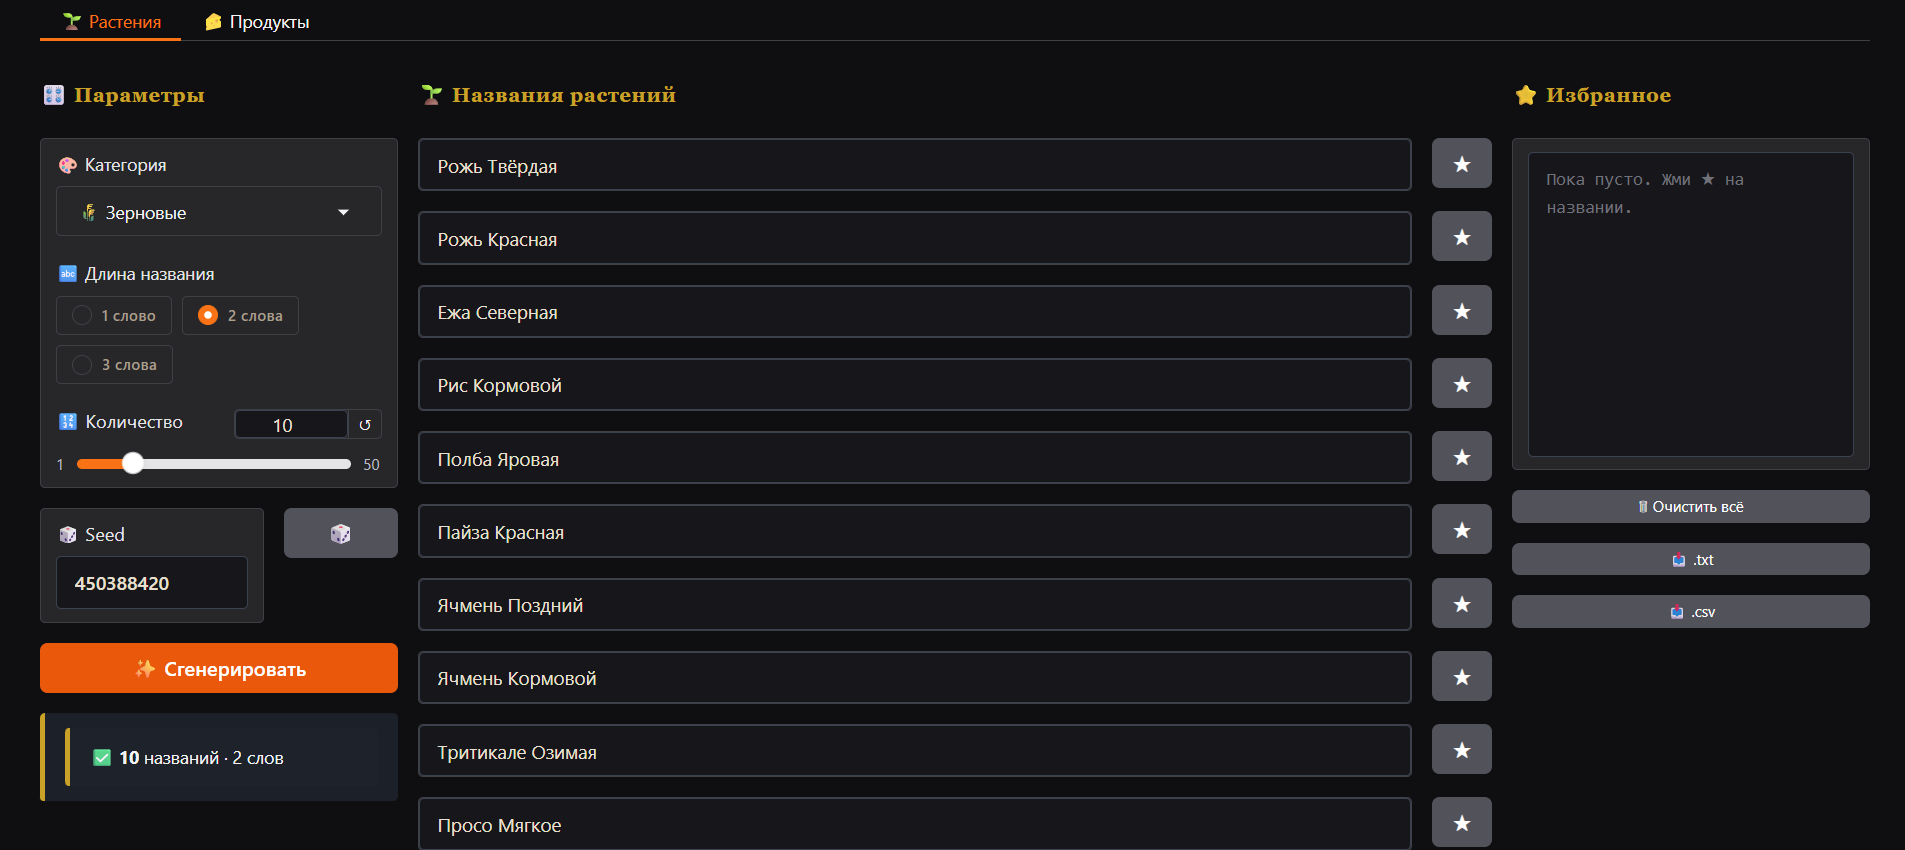
\includegraphics[width=\textwidth,keepaspectratio]{figures/image1.png}

\begin{center}\textbf{Рисунок 2.1 -- Вкладка «Растения» с результатами генерации}\end{center}

\noindent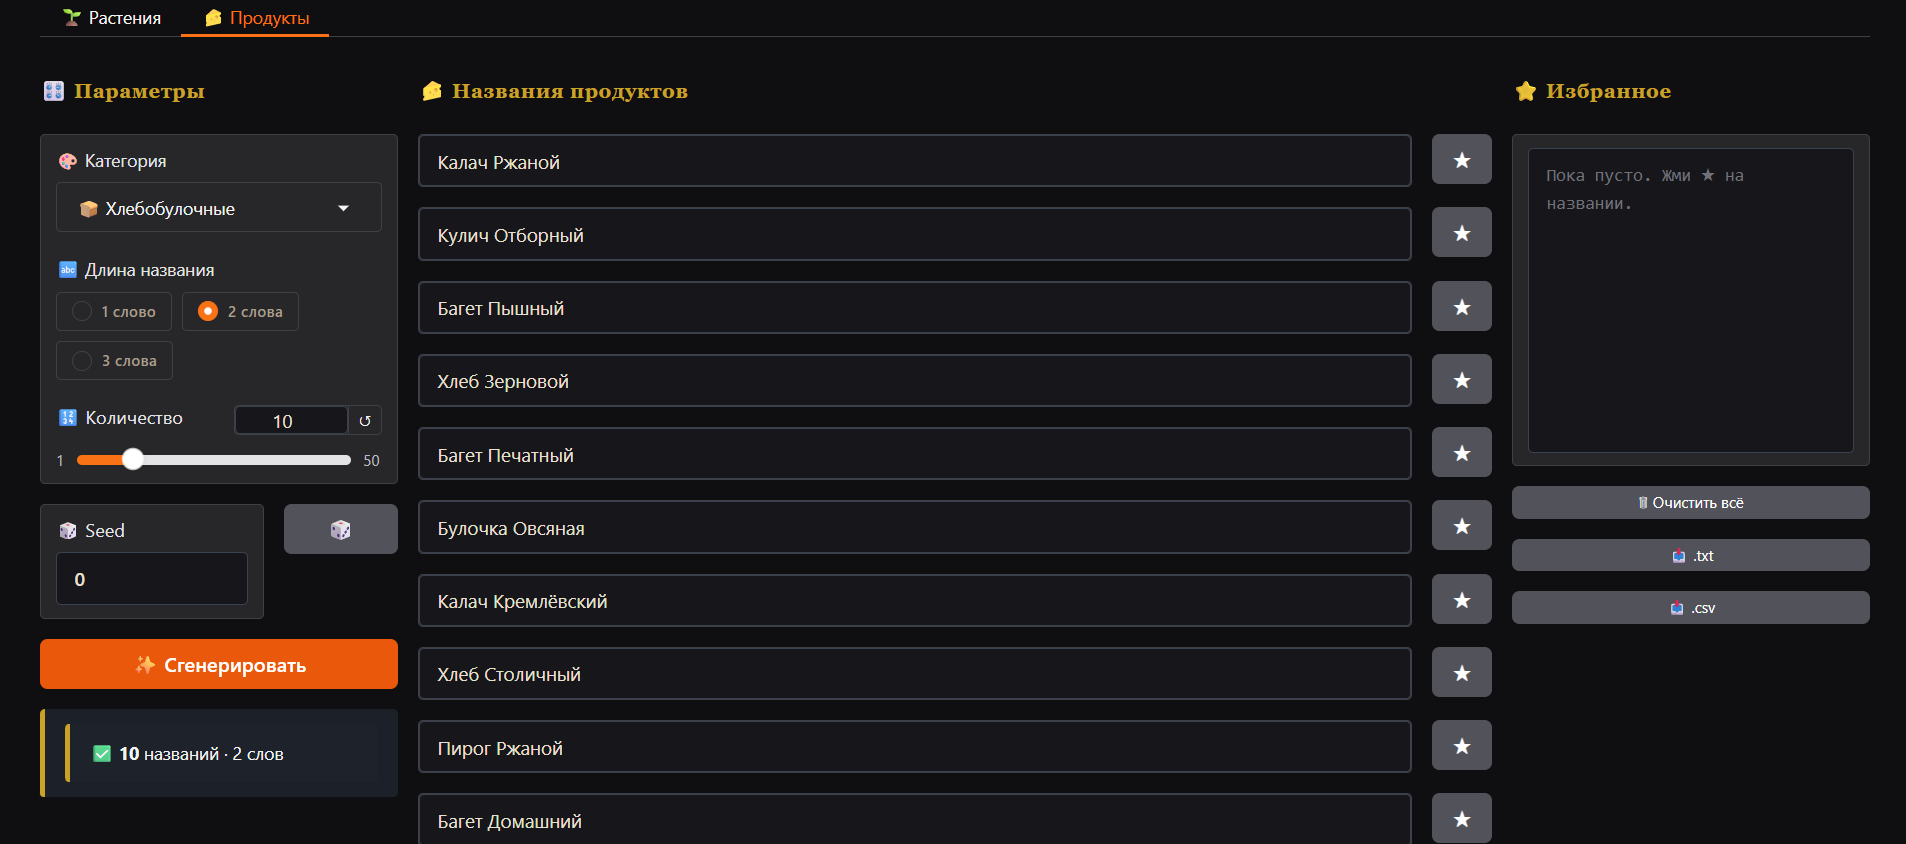
\includegraphics[width=\textwidth,keepaspectratio]{figures/image2.png}

\begin{center}\textbf{Рисунок 2.2 -- Вкладка «Продукты» с результатами генерации}\end{center}

В правой панели отображается избранное; данные растений и продуктов сохраняются отдельно. Пользователь может просматривать список, очищать его и экспортировать результаты.

Просмотреть список избранных названий.

Очистить список полностью (кнопка «Очистить всё»).

Экспортировать избранное в текстовый файл (.txt) или CSV-файл (.csv).

Файл .txt содержит по одному названию в строке, а CSV-файл -- столбец name. Оба формата подходят для дальнейшей обработки.

Избранное хранится в \path{user_data/plants_favorites.json} и \path{user_data/products_favorites.json}. Файлы создаются автоматически и сохраняются между запусками приложения.

Интерфейс оформлен в тёмной цветовой гамме с золотыми и багряными акцентами: тёмно-серый фон, контрастные панели и светлый текст.

Для распространения приложение собирается в .exe с помощью PyInstaller в режиме onedir: исполняемый файл и зависимости размещаются в одной папке. Такой вариант запускается быстрее, чем onefile, и удобен для копирования.

При первом запуске рядом с .exe создаётся папка user\_data для избранного и экспортированных файлов.

Приложение запускается за 3--5 секунд, генерация занимает менее секунды. Работа выполняется локально, без обращения к внешним сервисам.

Разработанный интерфейс объединяет основные функции системы: настройку параметров, просмотр результатов, избранное и экспорт. Приложение может использоваться локально на компьютере с Windows.

\chapter*{Заключение}\label{ux437ux430ux43aux43bux44eux447ux435ux43dux438ux435}
\addcontentsline{toc}{chapter}{Заключение}

\begin{spacing}{1.2}
\fontsize{13}{16.5}\selectfont
В курсовой работе рассмотрены методы машинного обучения для генерации названий растений и продуктов, а также разработано программное средство, объединяющее генеративную модель и модули оценки результатов. Теоретический анализ показал, что для небольшой специализированной предметной области рационально использовать компактную LSTM-модель: она учитывает контекст последовательности, обучается на центральном процессоре и не требует значительных вычислительных ресурсов.

Для обучения сформирован корпус названий растений и продуктов, проведены очистка, нормализация и удаление повторов. Дополнительно применена аугментация за счёт сочетания названий с прилагательными, что позволило увеличить объём обучающих данных примерно втрое. Для посимвольной LSTM реализовано условие по категории и длине названия; использованы два слоя, скрытое состояние размером 128, dropout 0,2 и оптимизатор Adam. Время обучения на CPU составляет около одной-двух минут.

Для отбора результатов разработаны три модуля скоринга: классификатор стиля на основе char-CNN, оценщик правдоподобия на основе биграммной языковой модели и оценщик новизны на основе n-граммного сравнения. В совокупности они ранжируют кандидатов и помогают выбирать варианты, соответствующие заданной категории. В ходе тестирования перплексия LSTM составила около 4--5 на валидационной выборке, а точность классификатора стилей достигла 80\%. Сравнение с марковской цепью и n-граммной моделью показало, что LSTM формирует более плавные и осмысленные названия.

Разработанный интерфейс на Gradio содержит отдельные вкладки для растений и продуктов. Пользователь может задать категорию, длину названия и количество вариантов, сохранить понравившиеся результаты в избранное и экспортировать их в текстовый или CSV-файл. Таким образом, поставленная цель достигнута: создано локальное приложение, пригодное для генерации названий в аграрных симуляторах, играх и прикладных задачах нейминга. Дальнейшую работу можно направить на расширение датасета, развитие словесных моделей с учётом морфологии и использование пользовательской обратной связи.
\end{spacing}

\chapter*{Библиографический список}\label{ux431ux438ux431ux43bux438ux43eux433ux440ux430ux444ux438ux447ux435ux441ux43aux438ux439-ux441ux43fux438ux441ux43eux43a}
\addcontentsline{toc}{chapter}{Библиографический список}

1. Гудфеллоу И., Бенджио И., Курвилль А. Глубокое обучение / пер. с англ. -- М.: ДМК Пресс, 2018. -- 652 с.

2. Николенко С., Кадурин А., Архангельская Е. Глубокое обучение. Погружение в мир нейронных сетей. -- СПб.: Питер, 2018. -- 480 с.

3. Хайкин С. Нейронные сети: полный курс. -- 2-е изд. -- М.: Вильямс, 2006. -- 1104 с.

4. Jurafsky D., Martin J. H. Speech and Language Processing. -- 3rd ed. -- Stanford University, 2023. -- 612 p.

5. Bengio Y., Ducharme R., Vincent P., Jauvin C. A Neural Probabilistic Language Model // Journal of Machine Learning Research. -- 2003. -- Vol. 3. -- P. 1137--1155.

6. Hochreiter S., Schmidhuber J. Long Short-Term Memory // Neural Computation. -- 1997. -- Vol. 9, No.~8. -- P. 1735--1780.

7. Sutskever I., Martens J., Hinton G. Generating Text with Recurrent Neural Networks // Proceedings of the 28th International Conference on Machine Learning (ICML). -- 2011. -- P. 1017--1024.

8. Karpathy A., Johnson J., Fei-Fei L. Visualizing and Understanding Recurrent Networks // International Conference on Learning Representations (ICLR) Workshop. -- 2016.

9. Zhang X., Zhao J., LeCun Y. Character-level Convolutional Networks for Text Classification // Advances in Neural Information Processing Systems (NIPS). -- 2015. -- Vol. 28. -- P. 649--657.

10. Kneser R., Ney H. Improved Backing-off for M-gram Language Modeling // Proceedings of the IEEE International Conference on Acoustics, Speech, and Signal Processing (ICASSP). -- 1995. -- Vol. 1. -- P. 181--184.

11. Vaswani A., Shazeer N., Parmar N. et al.~Attention Is All You Need // Advances in Neural Information Processing Systems (NIPS). -- 2017. -- Vol. 30. -- P. 5998--6008.

12. Kingma D. P., Ba J. Adam: A Method for Stochastic Optimization // International Conference on Learning Representations (ICLR). -- 2015.

13. Goodfellow I., Pouget-Abadie J., Mirza M. et al.~Generative Adversarial Nets // Advances in Neural Information Processing Systems (NIPS). -- 2014. -- Vol. 27. -- P. 2672--2680.

14. Srivastava N., Hinton G., Krizhevsky A. et al.~Dropout: A Simple Way to Prevent Neural Networks from Overfitting // Journal of Machine Learning Research. -- 2014. -- Vol. 15. -- P. 1929--1958.

15. Sundermeyer M., Schlüter R., Ney H. LSTM Neural Networks for Language Modeling // Proceedings of the 13th Annual Conference of the International Speech Communication Association (INTERSPEECH). -- 2012. -- P. 194--197.

16. Graves A. Generating Sequences With Recurrent Neural Networks // arXiv preprint arXiv:1308.0850. -- 2013.

17. Radford A., Wu J., Child R. et al.~Language Models are Unsupervised Multitask Learners // OpenAI Blog. -- 2019. -- Vol. 1, No.~8. -- P. 9.

18. Brown T. B., Mann B., Ryder N. et al.~Language Models are Few-Shot Learners // Advances in Neural Information Processing Systems (NeurIPS). -- 2020. -- Vol. 33. -- P. 1877--1901.

19. Рассел С., Норвиг П. Искусственный интеллект: современный подход. -- 4-е изд. -- М.: Вильямс, 2021. -- 1408 с.

20. Флах П. Машинное обучение. Наука и искусство построения алгоритмов, которые извлекают знания из данных. -- М.: ДМК Пресс, 2015. -- 400 с.

\chapter*{Приложение А}\label{ux43fux440ux438ux43bux43eux436ux435ux43dux438ux435-ux430}
\addcontentsline{toc}{chapter}{Приложение А}

\textbf{Листинг 3.1 -- фрагмент модуля предобработки названий}

\lstinputlisting{code/listing_05.py}

\chapter*{Приложение Б}\label{ux43fux440ux438ux43bux43eux436ux435ux43dux438ux435-ux431}
\addcontentsline{toc}{chapter}{Приложение Б}

\textbf{Листинг 3.2 -- фрагмент функции генерации названия}

\lstinputlisting{code/listing_06.py}

\chapter*{Приложение В}\label{ux43fux440ux438ux43bux43eux436ux435ux43dux438ux435-ux432}
\addcontentsline{toc}{chapter}{Приложение В}

\textbf{Листинг 3.3 -- фрагмент классификатора стилей}

\lstinputlisting{code/listing_07.py}

\chapter*{Приложение Г}\label{ux43fux440ux438ux43bux43eux436ux435ux43dux438ux435-ux433}
\addcontentsline{toc}{chapter}{Приложение Г}

\textbf{Листинг 3.4 -- фрагмент обработки запроса интерфейса}

\lstinputlisting[basicstyle=\ttfamily\fontsize{7.5}{7.8}\selectfont,aboveskip=8pt,belowskip=2pt]{code/listing_08.py}

\chapter*{Приложение Д}\label{ux43fux440ux438ux43bux43eux436ux435ux43dux438ux435-ux434}
\addcontentsline{toc}{chapter}{Приложение Д}

\textbf{Листинг 3.5 -- скрипт сборки .exe}

\lstinputlisting[basicstyle=\ttfamily\fontsize{8.2}{9.2}\selectfont]{code/listing_09.py}

\end{document}
